\documentclass[letterpaper, 12pt]{article}
\usepackage{color}
\usepackage{graphicx}
% Color boxes - nice
\usepackage[most]{tcolorbox}
% I like smaller margins
\usepackage[margin=1.0in]{geometry}
\begin{document}

\title{Notes on Single Dish Calibration}
\author{Dave Cohen}
\date{July 17, 2021}
\maketitle

\pagenumbering{roman}
\tableofcontents
\newpage
\pagenumbering{arabic}

\section{Introduction}
A successful radio telescope has been set up to observe the Hydrogen line at 1420.4 MHz. Recordings in both total power and spectral modes provide positive indication of Hydrogen with a manageable amount of RFI. The applications that are recording and displaying data are python scripts written by the author, based on the soapy SDR drivers. This was done because soapy supports multiple SDR platforms.

Despite being very useful, the measured values returned are not calibrated, returning power values in python \texttt{float64} format. It is desirable to have values that actually represent real world quantities.

Initial calculations have been performed with the Y-factor method {\color{red}(insert section ref)} to get an approxomation of the sytem temperature.  A directional coupler will later be installed to perform a more reliable ssytem calibration.  This is what many professional observatories do.

\section{Definitions}
Before addessing the problem, it is necessary to define the various quantities involved.

\begin{itemize}
	\item[-] \textbf{$\xi$}
	\\The system sensitivity, measured in $\frac{Jy}{Kelvin}$.
	\item[-] \textbf{k}
		\\Boltzman's constant, $1.38 * 10^{-23} \frac{Joules}{Kelvin}$
	\item[-] \textbf{$\theta$}
		\\The angular size of an object. {\color{red}(in degrees or radians?)}
	\item[-] \textbf{S}
		\\Flux density of object, in Janskys (Jy).
	\item[-] \textbf{T\textsubscript{sys}}
		\\System temperature, in degrees Kelvin. It is the total \textit{unwanted} power fed into the system which is the sum of the receiver temperature, the cold sky temperaure, and the ground or 'spillover` temperature.
	\item[-]\textbf{T\textsubscript{ND}}
		\\Noise diode temperature, in degrees Kelvin. This is the contribution of the noise diode which will be fed into the system.
\end{itemize}


\section{Determination of T\textsubscript{sys}}

\subsubsection{Y-factor Method}
This is probably the easiest way to determine T\textsubscript{sys}. The Y-factor equation:

\begin{equation}
Y = \frac{P_{cold}}{P_{hot}}
\end{equation}

P\textsubscript{cold} and P\textsubscript{hot} are determined by a pointing the antenna to a ''cold`` part of the sky with minimum hydrogen, then to a ''hot`` target, like nearby trees or the ground, both presumed to be at roughly 300 K. 
T\textsubscript{sys} is then determined by the following equation:

\begin{equation}
T_{sys} = \frac{T_{cold} - Y *T_{hot}}{Y - 1}
\end{equation}

\begin{figure}[h!]
	\centering
	%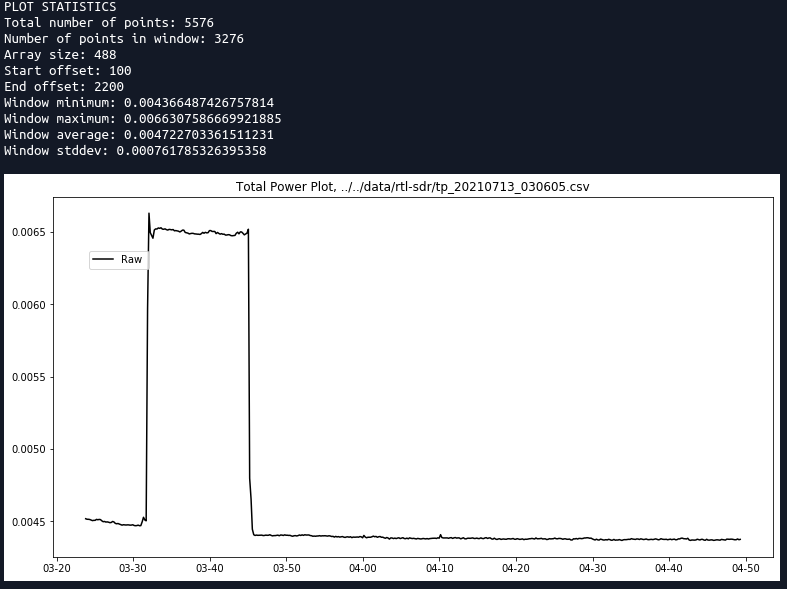
\includegraphics[width=1\textwidth]{tp_20210713_030605.png}
	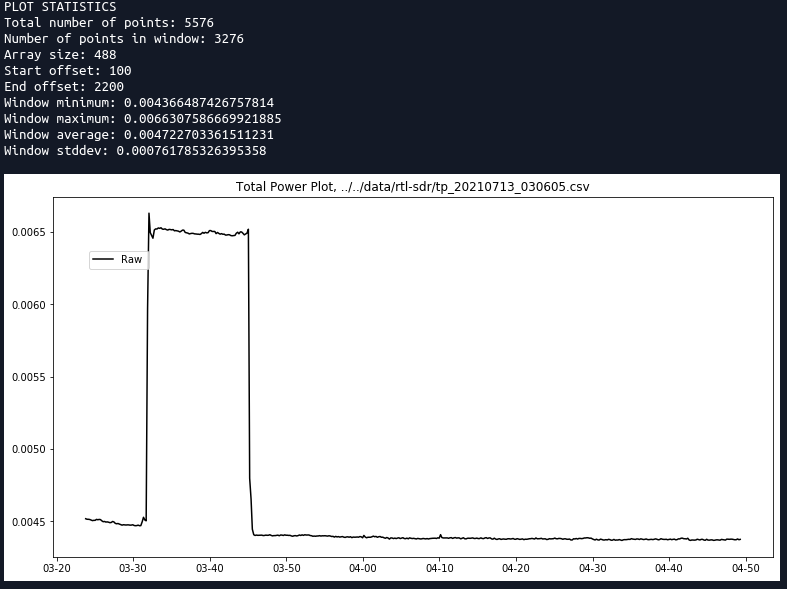
\includegraphics[scale = 0.5]{tp_20210713_030605.png}
	\label{tplot}
	\caption{Total power plot showing hot and cold measurement}
\end{figure}

The data were taken from a sample total power measurement, \ref{tplot}. The hot values were averaged over the time during which the hot measurement was in progress, roughly 0339 to 0343 UTC. The cold values are an average of the data for the time period 0410 to 0450 UTC.  

Plugging the values into equations (1) and (2):

$$Y = \frac{4.6163 * 10^{-6}}{1.0968 * 10^{-5}} = 0.42089 $$

$$T_{sys} = \frac{25 - 0.42089 * 300}{0.42089 - 1} = 174.87$$

Although the accuracy of this value is not certain, it falls in line with other sources. {\color{red}(referecnce SRT here)}

\subsection{Noise Source Injection}
This consists of injecting the signal from a noise source of known value into the receiver, typically through a directional coupler. The noise source can be attenuated to provide a calibration value that is suitable for the expected noise at the frequency of interest. For hydrogen measurements, this is typically around 10 K. {\color{red}(provide some proof)}  

\begin{figure}[h!]
	\centering
	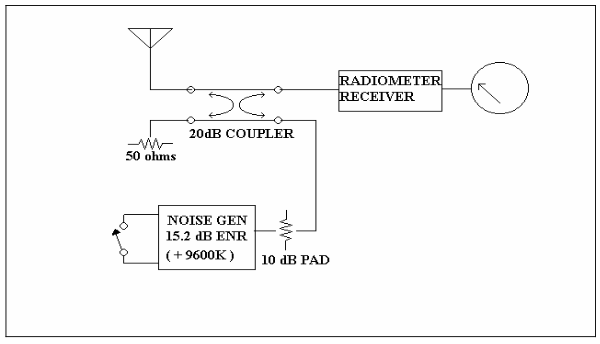
\includegraphics[scale=0.5]{dir_coupler.png}
	\caption{System using directional coupler for calibration}
	\label{coupler}
\end{figure}

Figure ~\ref{coupler} \cite{DCOUP} shows a noise source of 15.2 dB ENR, equivalent to 9600 K, as given by the following equation \cite{AN571}:

\begin{equation}
ENR_{dB} = 10 log (\frac{T_{hot} - T_{cold}}{T_{O}})
\end{equation}


ENR\textsubscript{dB} is the ratio, expressed in dB, of the difference between T\textsubscript{hot} and T\textsubscript{cold}, divided by 290K. T\textsubscript{cold} is assumed to be 290K when calibrated. So the noise source produces 9600K when on and 290K when off. It should also be noted that a 0 dB ENR noise source produces a 290K temperature change between its on and off states.

After the 10dB pad the signal is reduced by 10:1 to 960K noise. The coupler reduces the noise again by 20dB or 100:1, resulting in 9.6K added to the receiver input when the noise source is on. 

\begin{tcolorbox}[enhanced jigsaw,sharp corners,coltext=black,colback=lightgray,boxrule=0pt]
In the author's system, a 23dB coupler will be used, which reduces the noise by 200:1, resulting in a 4.6K addition to receiver noise. If the 4.6K noise addition proves insufficient, the attenuation of the pad can be reduced to increase the final added noise.
\end{tcolorbox}

\begin{figure}[h!]
	\centering
	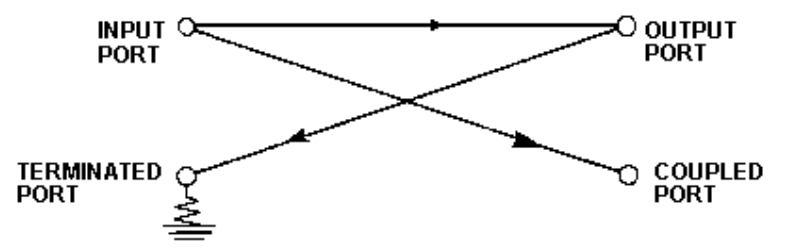
\includegraphics[scale=0.3]{threeport.png}
	\caption{Typical three-port coupler}
	\label{3PORT}
\end{figure}

Although not shown in Figure ~\ref{coupler}, a typical noise source would be a three-port device, as shown in Figure ~\ref{3PORT} {\color{red}(reference Mini-Circuits app note here)}. The fourth port is internally terminated to $50\Omega$. From Figure ~\ref{3PORT}, it can be inferred that the antenna would connect the output port, which is coupled to the terminated port. The input port, which is coupled to the coupled port, would connect to the LNA. That would allow both the antenna signal and the noise source to be presented to the LNA.

The equations to covert between decibels and power ratio:
$$dB = 10 * log(P)$$
$$P = 10^{\frac{dB}{10}}$$

What is of interest is the \textit{added} noise when the source is turned on.  For the authors system, the added noise would be 9602.8K. {\color{red}(is this right? look at it later)}
$$T_{added} = T_{hot} - 290K$$
$$T_{added} = 290 * 10^{\frac{ENR}{10}}$$

\begin{tcolorbox}[enhanced jigsaw,sharp corners,coltext=black,colback=lightgray,boxrule=0pt]
In the authors' setup, is was unclear exactly what ports to connect to. The coupler has an INPUT(J1) port, a COUPLED(J2) port, and an OUTPUT(J3) port. By experiment, I determined that the COUPLED port connects to the noise source and pad, the OUTPUT port connects to the antenna, and the INPUT port connects to the LNA. The isolated port, shown connected to a $50\Omega$ load, is internal to the device. I'm not sure what the effect is of reversing the connections to the INPUT and OUTPUT ports - I will determine that by experimentation, once the noise injection is completed.
\end{tcolorbox}

Once the added noise is known, T\textsubscript{sys} can be calculated based on the following equation:

\begin{equation}
R = (\frac{T_{sys} + T_{cal}}{T_{sys}})
\end{equation}

\section{Determination of Flux Density}
{\color{red}(reference Univ. Iowa Astromonical Laboratory 29:137, Fall 2007 here)}

Now that T\textsubscript{sys} is known, the flux density of a source can be determined by measuring the ratio of “on source” power to the “on” noise power (in both cases first subtract the Tsys contribution).

\begin{equation}
R = (\frac{\xi S}{T_{cal}})
\end{equation}

\newpage	% Put the bibliography on a new page
\begin{thebibliography}{10} % 10 is a random guess of the total number of
%references
\bibitem{AN571} Agilent Technologies, \emph{Fundamentals of Microwave Noise Figure Measurements, AN 57-1}, pp. 11-12.
\bibitem{DCOUP} Randall, B., \emph{Calibration Signal Injection with Directional Couplers}, 
Radio Astronomy, pp. 2-3, Jul-Aug 2005.
%\bibitem{MG} Goossens, M., Mittelbach, F., Samarin, \emph{A LaTeX
%Companion}, Addison-Wesley, Reading, MA, 1994.
%\bibitem{HK} Kopka, H., Daly P.W., \emph{A Guide to LaTeX},
%Addison-Wesley, Reading, MA, 1999.
%\bibitem{Pan} Pan, D., ``A Tutorial on MPEG/Audio Compression," \emph{IEEE
%Multimedia}, Vol.2, pp.60-74, Summer 1998.
\end{thebibliography}

\end{document}

%{\color{red}(referecnce Agilent Fundamentals of RF and Micorwave Noise Figure Measurements here, App. Note 57-1)}